% Options for packages loaded elsewhere
\PassOptionsToPackage{unicode}{hyperref}
\PassOptionsToPackage{hyphens}{url}
%
\documentclass[
  ignorenonframetext,
]{beamer}
\usepackage{pgfpages}
\setbeamertemplate{caption}[numbered]
\setbeamertemplate{caption label separator}{: }
\setbeamercolor{caption name}{fg=normal text.fg}
\beamertemplatenavigationsymbolsempty
% Prevent slide breaks in the middle of a paragraph
\widowpenalties 1 10000
\raggedbottom
\setbeamertemplate{part page}{
  \centering
  \begin{beamercolorbox}[sep=16pt,center]{part title}
    \usebeamerfont{part title}\insertpart\par
  \end{beamercolorbox}
}
\setbeamertemplate{section page}{
  \centering
  \begin{beamercolorbox}[sep=12pt,center]{part title}
    \usebeamerfont{section title}\insertsection\par
  \end{beamercolorbox}
}
\setbeamertemplate{subsection page}{
  \centering
  \begin{beamercolorbox}[sep=8pt,center]{part title}
    \usebeamerfont{subsection title}\insertsubsection\par
  \end{beamercolorbox}
}
\AtBeginPart{
  \frame{\partpage}
}
\AtBeginSection{
  \ifbibliography
  \else
    \frame{\sectionpage}
  \fi
}
\AtBeginSubsection{
  \frame{\subsectionpage}
}
\usepackage{lmodern}
\usepackage{amssymb,amsmath}
\usepackage{ifxetex,ifluatex}
\ifnum 0\ifxetex 1\fi\ifluatex 1\fi=0 % if pdftex
  \usepackage[T1]{fontenc}
  \usepackage[utf8]{inputenc}
  \usepackage{textcomp} % provide euro and other symbols
\else % if luatex or xetex
  \usepackage{unicode-math}
  \defaultfontfeatures{Scale=MatchLowercase}
  \defaultfontfeatures[\rmfamily]{Ligatures=TeX,Scale=1}
\fi
% Use upquote if available, for straight quotes in verbatim environments
\IfFileExists{upquote.sty}{\usepackage{upquote}}{}
\IfFileExists{microtype.sty}{% use microtype if available
  \usepackage[]{microtype}
  \UseMicrotypeSet[protrusion]{basicmath} % disable protrusion for tt fonts
}{}
\makeatletter
\@ifundefined{KOMAClassName}{% if non-KOMA class
  \IfFileExists{parskip.sty}{%
    \usepackage{parskip}
  }{% else
    \setlength{\parindent}{0pt}
    \setlength{\parskip}{6pt plus 2pt minus 1pt}}
}{% if KOMA class
  \KOMAoptions{parskip=half}}
\makeatother
\usepackage{xcolor}
\IfFileExists{xurl.sty}{\usepackage{xurl}}{} % add URL line breaks if available
\IfFileExists{bookmark.sty}{\usepackage{bookmark}}{\usepackage{hyperref}}
\hypersetup{
  pdftitle={GLM I - Estimating Parameter Accuracy},
  hidelinks,
  pdfcreator={LaTeX via pandoc}}
\urlstyle{same} % disable monospaced font for URLs
\newif\ifbibliography
\usepackage{color}
\usepackage{fancyvrb}
\newcommand{\VerbBar}{|}
\newcommand{\VERB}{\Verb[commandchars=\\\{\}]}
\DefineVerbatimEnvironment{Highlighting}{Verbatim}{commandchars=\\\{\}}
% Add ',fontsize=\small' for more characters per line
\usepackage{framed}
\definecolor{shadecolor}{RGB}{248,248,248}
\newenvironment{Shaded}{\begin{snugshade}}{\end{snugshade}}
\newcommand{\AlertTok}[1]{\textcolor[rgb]{0.94,0.16,0.16}{#1}}
\newcommand{\AnnotationTok}[1]{\textcolor[rgb]{0.56,0.35,0.01}{\textbf{\textit{#1}}}}
\newcommand{\AttributeTok}[1]{\textcolor[rgb]{0.77,0.63,0.00}{#1}}
\newcommand{\BaseNTok}[1]{\textcolor[rgb]{0.00,0.00,0.81}{#1}}
\newcommand{\BuiltInTok}[1]{#1}
\newcommand{\CharTok}[1]{\textcolor[rgb]{0.31,0.60,0.02}{#1}}
\newcommand{\CommentTok}[1]{\textcolor[rgb]{0.56,0.35,0.01}{\textit{#1}}}
\newcommand{\CommentVarTok}[1]{\textcolor[rgb]{0.56,0.35,0.01}{\textbf{\textit{#1}}}}
\newcommand{\ConstantTok}[1]{\textcolor[rgb]{0.00,0.00,0.00}{#1}}
\newcommand{\ControlFlowTok}[1]{\textcolor[rgb]{0.13,0.29,0.53}{\textbf{#1}}}
\newcommand{\DataTypeTok}[1]{\textcolor[rgb]{0.13,0.29,0.53}{#1}}
\newcommand{\DecValTok}[1]{\textcolor[rgb]{0.00,0.00,0.81}{#1}}
\newcommand{\DocumentationTok}[1]{\textcolor[rgb]{0.56,0.35,0.01}{\textbf{\textit{#1}}}}
\newcommand{\ErrorTok}[1]{\textcolor[rgb]{0.64,0.00,0.00}{\textbf{#1}}}
\newcommand{\ExtensionTok}[1]{#1}
\newcommand{\FloatTok}[1]{\textcolor[rgb]{0.00,0.00,0.81}{#1}}
\newcommand{\FunctionTok}[1]{\textcolor[rgb]{0.00,0.00,0.00}{#1}}
\newcommand{\ImportTok}[1]{#1}
\newcommand{\InformationTok}[1]{\textcolor[rgb]{0.56,0.35,0.01}{\textbf{\textit{#1}}}}
\newcommand{\KeywordTok}[1]{\textcolor[rgb]{0.13,0.29,0.53}{\textbf{#1}}}
\newcommand{\NormalTok}[1]{#1}
\newcommand{\OperatorTok}[1]{\textcolor[rgb]{0.81,0.36,0.00}{\textbf{#1}}}
\newcommand{\OtherTok}[1]{\textcolor[rgb]{0.56,0.35,0.01}{#1}}
\newcommand{\PreprocessorTok}[1]{\textcolor[rgb]{0.56,0.35,0.01}{\textit{#1}}}
\newcommand{\RegionMarkerTok}[1]{#1}
\newcommand{\SpecialCharTok}[1]{\textcolor[rgb]{0.00,0.00,0.00}{#1}}
\newcommand{\SpecialStringTok}[1]{\textcolor[rgb]{0.31,0.60,0.02}{#1}}
\newcommand{\StringTok}[1]{\textcolor[rgb]{0.31,0.60,0.02}{#1}}
\newcommand{\VariableTok}[1]{\textcolor[rgb]{0.00,0.00,0.00}{#1}}
\newcommand{\VerbatimStringTok}[1]{\textcolor[rgb]{0.31,0.60,0.02}{#1}}
\newcommand{\WarningTok}[1]{\textcolor[rgb]{0.56,0.35,0.01}{\textbf{\textit{#1}}}}
\usepackage{longtable,booktabs}
\usepackage{caption}
% Make caption package work with longtable
\makeatletter
\def\fnum@table{\tablename~\thetable}
\makeatother
\setlength{\emergencystretch}{3em} % prevent overfull lines
\providecommand{\tightlist}{%
  \setlength{\itemsep}{0pt}\setlength{\parskip}{0pt}}
\setcounter{secnumdepth}{-\maxdimen} % remove section numbering

\title{GLM I - Estimating Parameter Accuracy}
\subtitle{September 10th, 2020}
\author{}
\date{\vspace{-2.5em}}

\begin{document}
\frame{\titlepage}

\begin{frame}{Review Homework}
\protect\hypertarget{review-homework}{}

\begin{enumerate}
\tightlist
\item
  Make sure to submit the assigment when you are done
\item
  The plot was not useful because of overplotting - it's ok to have a
  plot that does not show any relationship
\item
  If you use r markdown please submit the rendered document - not the
  raw .Rmd
\item
  There seems to be a problem with .html files - I think you have to zip
  them prior to submitting
\end{enumerate}

\end{frame}

\hypertarget{parameter-accuracy}{%
\section{Parameter Accuracy}\label{parameter-accuracy}}

\begin{frame}{Where we are:}
\protect\hypertarget{where-we-are}{}

\[
Y = \beta_0 + \beta_1X
\]

\[
\begin{aligned}
\hat\beta_0 &= \bar{Y} - \hat\beta_1\bar{X} \\
\hat\beta_1 &= \frac{\sum{(X_i - \bar{X})(Y_i - \bar{Y})}}{\sum{(X_i - \bar{X})^2}} \\
\hat{\sigma}^2 &= \frac{\sum{(Y_i - \hat{Y_i})^2}}{n-2}
\end{aligned}
\]

\end{frame}

\begin{frame}{How confident are we in these values?}
\protect\hypertarget{how-confident-are-we-in-these-values}{}

\end{frame}

\begin{frame}[fragile]{Sampling Distribution of \(\hat\beta_1\)}
\protect\hypertarget{sampling-distribution-of-hatbeta_1}{}

\[
E\{\beta_1\} = \hat{\beta_1} \\
\sigma^2\{\beta_1\} = \frac{\hat\sigma^2}{\sum{(X_i - \bar{X})^2}}
\]

\begin{itemize}
\tightlist
\item
  where we use the unbiased estimate of \(\sigma^2\) from before.
\end{itemize}

\begin{Shaded}
\begin{Highlighting}[]
\NormalTok{sigma_beta_}\DecValTok{1}\NormalTok{ <-}\StringTok{ }\KeywordTok{sqrt}\NormalTok{(sigma}\OperatorTok{^}\DecValTok{2}\OperatorTok{/}\KeywordTok{sum}\NormalTok{((peng}\OperatorTok{$}\NormalTok{body_mass_g }\OperatorTok{-}\StringTok{ }\KeywordTok{mean}\NormalTok{(peng}\OperatorTok{$}\NormalTok{body_mass_g))}\OperatorTok{^}\DecValTok{2}\NormalTok{))}
\end{Highlighting}
\end{Shaded}

\begin{itemize}
\item
  The normality of the sampling distribution of \(\hat\beta_1\) follows
  from the fact that \(\hat\beta_1\) is a linear combination of \(Y_i\)
\item
  What happens when we get more data?
\end{itemize}

\end{frame}

\begin{frame}{Standardized sample distirbution for \(\hat\beta_1\)}
\protect\hypertarget{standardized-sample-distirbution-for-hatbeta_1}{}

\begin{itemize}
\tightlist
\item
  The standardized distribution follows a t distribution with n-2
  degrees of freedom
\end{itemize}

\[
\frac{\hat\beta_1 - E\{\hat\beta_1\}}{\hat\sigma^2\{\hat\beta_1\}} \sim t(n-2) 
\] - \(t\) distribution is necessary because we are estimating the
variance in denominator

\end{frame}

\begin{frame}{Creating confidence intervals for \(\hat\beta_1\)}
\protect\hypertarget{creating-confidence-intervals-for-hatbeta_1}{}

set \(\alpha = .95\)

\[
\hat\beta_1 + \hat\sigma * t(\frac{1-\alpha}{2}, n - 2) \\
\hat\beta_1 + \hat\sigma * t(\frac{1+\alpha}{2}, n - 2)
\]

\begin{center}\includegraphics[width=0.5\linewidth]{Class-02-Estimating-Accuracy_files/figure-beamer/unnamed-chunk-3-1} \end{center}

\end{frame}

\begin{frame}[fragile]{Example with \(\beta_1\)}
\protect\hypertarget{example-with-beta_1}{}

\begin{Shaded}
\begin{Highlighting}[]
\NormalTok{low_}\DecValTok{95}\NormalTok{_ci <-}\StringTok{ }\NormalTok{beta1 }\OperatorTok{+}\StringTok{ }\NormalTok{sigma_beta_}\DecValTok{1}\OperatorTok{*}\KeywordTok{qt}\NormalTok{(.}\DecValTok{025}\NormalTok{, }\DataTypeTok{df =} \KeywordTok{nrow}\NormalTok{(peng) }\OperatorTok{-}\StringTok{ }\DecValTok{2}\NormalTok{)}
\NormalTok{high_}\DecValTok{95}\NormalTok{_ci <-}\StringTok{ }\NormalTok{beta1 }\OperatorTok{+}\StringTok{ }\NormalTok{sigma_beta_}\DecValTok{1}\OperatorTok{*}\KeywordTok{qt}\NormalTok{(.}\DecValTok{975}\NormalTok{, }\DataTypeTok{df =} \KeywordTok{nrow}\NormalTok{(peng) }\OperatorTok{-}\StringTok{ }\DecValTok{2}\NormalTok{)}
\end{Highlighting}
\end{Shaded}

\begin{center}\includegraphics{Class-02-Estimating-Accuracy_files/figure-beamer/unnamed-chunk-5-1} \end{center}

\end{frame}

\begin{frame}{Interpertaion of confidence interval}
\protect\hypertarget{interpertaion-of-confidence-interval}{}

\begin{itemize}
\tightlist
\item
  It is not:

  \begin{itemize}
  \tightlist
  \item
    The true value of \(\beta_1\) has a 95\% chance of falling between
    the low and high value
  \end{itemize}
\item
  More accurate:

  \begin{itemize}
  \tightlist
  \item
    If you repeat the experiment, you expect that 95\% of the CIs
    contain the true value of \(beta_1\)
  \end{itemize}
\end{itemize}

\end{frame}

\begin{frame}[fragile]{Sampling Distribution of \(\hat\beta_0\)}
\protect\hypertarget{sampling-distribution-of-hatbeta_0}{}

\[
E\{\beta_0\} = \hat{\beta_0} \\
\sigma^2\{\beta_0\} = \hat\sigma^2  \left[\frac{1}{n} +  \frac{\bar{X}^2}{\sum{(X_i - \bar{X})^2}} \right]
\]

\begin{Shaded}
\begin{Highlighting}[]
\NormalTok{sigma_beta_}\DecValTok{0}\NormalTok{ <-}\StringTok{ }\KeywordTok{sqrt}\NormalTok{(sigma}\OperatorTok{^}\DecValTok{2}\OperatorTok{*}\NormalTok{(}\DecValTok{1}\OperatorTok{/}\KeywordTok{nrow}\NormalTok{(peng) }\OperatorTok{+}\StringTok{ }\KeywordTok{mean}\NormalTok{(peng}\OperatorTok{$}\NormalTok{body_mass_g)}\OperatorTok{^}\DecValTok{2}\OperatorTok{/}
\StringTok{                                }\KeywordTok{sum}\NormalTok{((peng}\OperatorTok{$}\NormalTok{body_mass_g }\OperatorTok{-}\StringTok{ }\KeywordTok{mean}\NormalTok{(peng}\OperatorTok{$}\NormalTok{body_mass_g))}\OperatorTok{^}\DecValTok{2}\NormalTok{)))}
\end{Highlighting}
\end{Shaded}

\end{frame}

\begin{frame}{Sampling Distribution Around \(\hat{Y}\)}
\protect\hypertarget{sampling-distribution-around-haty}{}

\[
E\{\hat{Y}_h\} = \hat{\beta_0} + \hat\beta_1X_h \\
\sigma^2\{\hat{Y}_h\} = \hat\sigma^2  \left[\frac{1}{n} +  \frac{(X_h - \bar{X})^2}{\sum{(X_i - \bar{X})^2}} \right]
\]

\begin{itemize}
\tightlist
\item
  What happens when X\_h = 0?
\item
  What happens when we are far from \(\bar{X}\)?
\end{itemize}

\end{frame}

\begin{frame}{Distribution for \(\hat{Y}\)}
\protect\hypertarget{distribution-for-haty}{}

\begin{center}\includegraphics{Class-02-Estimating-Accuracy_files/figure-beamer/unnamed-chunk-7-1} \end{center}

\end{frame}

\begin{frame}{Sampling Distribution around new observation (prediction)}
\protect\hypertarget{sampling-distribution-around-new-observation-prediction}{}

\[
E\{\hat{Y}_{new}\} = \hat{\beta_0} + \hat\beta_1X_h \\
\sigma^2\{\hat{Y}_{new}\} = \hat\sigma^2  \left[1 + \frac{1}{n} +  \frac{(X_h - \bar{X})^2}{\sum{(X_i - \bar{X})^2}} \right]
\]

\end{frame}

\begin{frame}{Sampling Distribution around new observation (prediction)}
\protect\hypertarget{sampling-distribution-around-new-observation-prediction-1}{}

\begin{itemize}
\tightlist
\item
  if you have \(m\) new observations at a given \(X_h\)
\end{itemize}

\[
\sigma^2\{\hat{Y}_{new_m}\} = \hat\sigma^2  \left[\frac{1}{m} + \frac{1}{n} +  \frac{(X_h - \bar{X})^2}{\sum{(X_i - \bar{X})^2}} \right]
\]

\begin{center}\includegraphics[width=0.6\linewidth]{Class-02-Estimating-Accuracy_files/figure-beamer/unnamed-chunk-8-1} \end{center}

\end{frame}

\hypertarget{hypothesis-test}{%
\section{Hypothesis Test}\label{hypothesis-test}}

\begin{frame}{Setup}
\protect\hypertarget{setup}{}

\begin{itemize}
\tightlist
\item
  We often wish to determine the significance of a variable or multiple
  variables. We must create a null hypothesis and an alternative
  hypothesis to test
\end{itemize}

\[
H_0: \beta_1 = 0 \\
H_a: \beta_1 \neq 0
\] We set an alpha level which is the probability of rejecting the null
hypothesis given that it's true. Columns show what is true:

\begin{longtable}[]{@{}lll@{}}
\toprule
Study Says & \(H_0\) & \(H_a\)\tabularnewline
\midrule
\endhead
No effect & Correct & Type II (\(\beta\))\tabularnewline
Effect & Type I (\(\alpha\)) & Correct\tabularnewline
\bottomrule
\end{longtable}

\end{frame}

\begin{frame}{How to set \(\alpha\)?}
\protect\hypertarget{how-to-set-alpha}{}

\begin{itemize}
\tightlist
\item
  Often times alpha is set at .05
\item
  However it should depend on the application used
\item
  How bad is it if you say there is an effect when there isn't one?
\end{itemize}

\end{frame}

\begin{frame}{What about \(\beta\)?}
\protect\hypertarget{what-about-beta}{}

\begin{itemize}
\tightlist
\item
  This is related to your ability to detect an effect
\item
  What are the two things that influence this (given a model)?
\end{itemize}

\end{frame}

\begin{frame}{P value}
\protect\hypertarget{p-value}{}

\begin{itemize}
\tightlist
\item
  The probability that you observe data at least as extreme as yours
  given the null hypothesis
\item
  This is not the probability that your null hypothesis is true because
  you are assuming it already is
\end{itemize}

A low p value can happen:

\begin{itemize}
\tightlist
\item
  The null is true but your sample is unusual
\item
  the null is false
\end{itemize}

\end{frame}

\begin{frame}[fragile]{Calculating the p-value for the hypothesis above}
\protect\hypertarget{calculating-the-p-value-for-the-hypothesis-above}{}

\[
\frac{\hat\beta_1 - E\{\hat\beta_1\}}{\hat\sigma^2\{\hat\beta_1\}} \sim t(n-2) 
\]

if \(H_0\) is true then \(E\{\hat\beta_1\} = 0\) therefore:

\[
\frac{\hat\beta_1}{\hat\sigma^2\{\hat\beta_1\}} \sim t(n-2) 
\]

\begin{Shaded}
\begin{Highlighting}[]
\KeywordTok{pt}\NormalTok{(}\KeywordTok{abs}\NormalTok{(beta1}\OperatorTok{/}\NormalTok{sigma_beta_}\DecValTok{1}\OperatorTok{^}\DecValTok{2}\NormalTok{), }\DataTypeTok{df =} \KeywordTok{nrow}\NormalTok{(peng) }\OperatorTok{-}\StringTok{ }\DecValTok{2}\NormalTok{, }\DataTypeTok{lower.tail =} \OtherTok{FALSE}\NormalTok{)}\OperatorTok{*}\DecValTok{2}
\end{Highlighting}
\end{Shaded}

\begin{verbatim}
## body_mass_g 
##           0
\end{verbatim}

\end{frame}

\begin{frame}[fragile]{Create a fake variable for illustration}
\protect\hypertarget{create-a-fake-variable-for-illustration}{}

\begin{Shaded}
\begin{Highlighting}[]
\NormalTok{fake_est}
\end{Highlighting}
\end{Shaded}

\begin{verbatim}
## fake_random 
##   -0.889426
\end{verbatim}

\begin{Shaded}
\begin{Highlighting}[]
\NormalTok{fake_est_se}
\end{Highlighting}
\end{Shaded}

\begin{verbatim}
## [1] 0.7354721
\end{verbatim}

\begin{Shaded}
\begin{Highlighting}[]
\NormalTok{fake_est}\OperatorTok{/}\NormalTok{fake_est_se}
\end{Highlighting}
\end{Shaded}

\begin{verbatim}
## fake_random 
##   -1.209327
\end{verbatim}

\begin{Shaded}
\begin{Highlighting}[]
\KeywordTok{pt}\NormalTok{(fake_est}\OperatorTok{/}\NormalTok{fake_est_se, }\DataTypeTok{df =} \KeywordTok{nrow}\NormalTok{(peng) }\OperatorTok{-}\StringTok{ }\DecValTok{2}\NormalTok{, }\DataTypeTok{lower.tail =} \OtherTok{TRUE}\NormalTok{) }\OperatorTok{*}\StringTok{ }\DecValTok{2}
\end{Highlighting}
\end{Shaded}

\begin{verbatim}
## fake_random 
##   0.2274004
\end{verbatim}

\begin{itemize}
\tightlist
\item
  This gives the same values as the F test for a single variable (see
  reading)
\end{itemize}

\end{frame}

\begin{frame}{Why double?}
\protect\hypertarget{why-double}{}

\begin{itemize}
\tightlist
\item
  We aren't assuming a direction sowe have to check both sides of the
  t-distribution
\end{itemize}

\begin{center}\includegraphics{Class-02-Estimating-Accuracy_files/figure-beamer/unnamed-chunk-13-1} \end{center}

\end{frame}

\hypertarget{diagnostics}{%
\section{Diagnostics}\label{diagnostics}}

\begin{frame}{R Squared}
\protect\hypertarget{r-squared}{}

\begin{itemize}
\tightlist
\item
  The \(R^2\), also called the coefficient of determination or
  percentage of variance explained:
\end{itemize}

\[
R^2 = 1 - \frac{\sum(\hat{y}_i - y_i)^2}{\sum(\bar{y}_i - y_i)^2} = 1 - \frac{RSS}{TSS}
\] - What kind of model definition means that \(\bar{y} =\hat{y}\)?

\end{frame}

\begin{frame}{\(R^2\) - what is it good for?}
\protect\hypertarget{r2---what-is-it-good-for}{}

\begin{itemize}
\tightlist
\item
  Correlation between \(\hat{y}\) and \(X\)
\item
  Anscombe's Quartet - R\^{}2 is the same for all
\end{itemize}

\begin{center}\includegraphics{Class-02-Estimating-Accuracy_files/figure-beamer/unnamed-chunk-14-1} \end{center}

\end{frame}

\begin{frame}{\(R^2\) words of caution}
\protect\hypertarget{r2-words-of-caution}{}

\begin{itemize}
\tightlist
\item
  Always improves with more predictors (number of predictors: \(p\))
\end{itemize}

\[
R_a^2 = 1 - \frac{RSS/(n-p)}{TSS/(n-1)}
\]

\begin{itemize}
\tightlist
\item
  Is not easily generalized to other types of models - the deviance is
  more general.
\item
  For the linear model the deviance is the RSS
\end{itemize}

\end{frame}

\begin{frame}{Residuals}
\protect\hypertarget{residuals}{}

\begin{itemize}
\tightlist
\item
  In my opinion the best way to diagnose model issues
\item
  Make sure nothing totally wrong is happening
\end{itemize}

\end{frame}

\begin{frame}{Residuals \textbar{} predictor variable (1)}
\protect\hypertarget{residuals-predictor-variable-1}{}

\begin{center}\includegraphics{Class-02-Estimating-Accuracy_files/figure-beamer/unnamed-chunk-16-1} \end{center}

\end{frame}

\begin{frame}[fragile]{Residuals \textbar{} predictor variable (2)}
\protect\hypertarget{residuals-predictor-variable-2}{}

\begin{Shaded}
\begin{Highlighting}[]
\NormalTok{bill_length_mod <-}\StringTok{ }\KeywordTok{lm}\NormalTok{(bill_length_mm }\OperatorTok{~}\StringTok{ }\NormalTok{body_mass_g, }\DataTypeTok{data =}\NormalTok{ peng)}
\NormalTok{bill_length_residuals <-}\StringTok{ }\KeywordTok{residuals}\NormalTok{(bill_length_mod)}
\end{Highlighting}
\end{Shaded}

\begin{center}\includegraphics{Class-02-Estimating-Accuracy_files/figure-beamer/unnamed-chunk-18-1} \end{center}

\end{frame}

\begin{frame}{Residuals\textbar{} Fitted Values}
\protect\hypertarget{residuals-fitted-values}{}

\begin{center}\includegraphics{Class-02-Estimating-Accuracy_files/figure-beamer/unnamed-chunk-19-1} \end{center}

\end{frame}

\begin{frame}{Residuals \textbar{} Normal Q-Q Plot}
\protect\hypertarget{residuals-normal-q-q-plot}{}

\begin{itemize}
\tightlist
\item
  Standardized residuals
\end{itemize}

\[
var(\hat\epsilon) = \hat\sigma^2(1-h_{ii})
\] where \(h_ii\) is the leverage of a point which is defined as:

\[
Hy = X(X'X)^{-1}X'y = \hat y
\]

\begin{center}\includegraphics[width=0.4\linewidth]{Class-02-Estimating-Accuracy_files/figure-beamer/unnamed-chunk-20-1} \end{center}

\end{frame}

\begin{frame}{Residuals \textbar{} Against other predictor}
\protect\hypertarget{residuals-against-other-predictor}{}

\begin{center}\includegraphics{Class-02-Estimating-Accuracy_files/figure-beamer/unnamed-chunk-21-1} \end{center}

\end{frame}

\hypertarget{extending-the-ordinary-model}{%
\section{Extending the ordinary
model}\label{extending-the-ordinary-model}}

\begin{frame}{Let's add predictors}
\protect\hypertarget{lets-add-predictors}{}

\[
Y = \beta_0 + \beta_1X_1 + \beta_2X_2 + \cdots + \beta_{p-1}X_{p-1} +\beta_pX_p 
\]

\end{frame}

\begin{frame}[fragile]{Add species as another variable \textbar{}
original model}
\protect\hypertarget{add-species-as-another-variable-original-model}{}

\begin{Shaded}
\begin{Highlighting}[]
\NormalTok{model1 <-}\StringTok{ }\KeywordTok{lm}\NormalTok{(flipper_length_mm }\OperatorTok{~}\StringTok{ }\NormalTok{body_mass_g, }\DataTypeTok{data =}\NormalTok{ peng)}
\KeywordTok{summary}\NormalTok{(model1)}
\end{Highlighting}
\end{Shaded}

\begin{verbatim}
## 
## Call:
## lm(formula = flipper_length_mm ~ body_mass_g, data = peng)
## 
## Residuals:
##     Min      1Q  Median      3Q     Max 
## -23.698  -4.983   1.056   5.101  13.933 
## 
## Coefficients:
##              Estimate Std. Error t value Pr(>|t|)    
## (Intercept) 1.370e+02  1.999e+00   68.56   <2e-16 ***
## body_mass_g 1.520e-02  4.667e-04   32.56   <2e-16 ***
## ---
## Signif. codes:  0 '***' 0.001 '**' 0.01 '*' 0.05 '.' 0.1 ' ' 1
## 
## Residual standard error: 6.847 on 331 degrees of freedom
## Multiple R-squared:  0.7621, Adjusted R-squared:  0.7614 
## F-statistic:  1060 on 1 and 331 DF,  p-value: < 2.2e-16
\end{verbatim}

\end{frame}

\begin{frame}[fragile]{Add species as another variable \textbar{} adding
species}
\protect\hypertarget{add-species-as-another-variable-adding-species}{}

\begin{Shaded}
\begin{Highlighting}[]
\NormalTok{model2 <-}\StringTok{ }\KeywordTok{lm}\NormalTok{(flipper_length_mm }\OperatorTok{~}\StringTok{ }\NormalTok{body_mass_g }\OperatorTok{+}\StringTok{ }\NormalTok{species, }\DataTypeTok{data =}\NormalTok{ peng)}
\KeywordTok{summary}\NormalTok{(model2)}
\end{Highlighting}
\end{Shaded}

\begin{verbatim}
## 
## Call:
## lm(formula = flipper_length_mm ~ body_mass_g + species, data = peng)
## 
## Residuals:
##      Min       1Q   Median       3Q      Max 
## -14.5418  -3.1804   0.0983   3.3295  17.3954 
## 
## Coefficients:
##                   Estimate Std. Error t value Pr(>|t|)    
## (Intercept)      1.585e+02  2.435e+00  65.119  < 2e-16 ***
## body_mass_g      8.515e-03  6.457e-04  13.186  < 2e-16 ***
## speciesChinstrap 5.492e+00  7.938e-01   6.918  2.4e-11 ***
## speciesGentoo    1.533e+01  1.117e+00  13.727  < 2e-16 ***
## ---
## Signif. codes:  0 '***' 0.001 '**' 0.01 '*' 0.05 '.' 0.1 ' ' 1
## 
## Residual standard error: 5.405 on 329 degrees of freedom
## Multiple R-squared:  0.8526, Adjusted R-squared:  0.8513 
## F-statistic: 634.4 on 3 and 329 DF,  p-value: < 2.2e-16
\end{verbatim}

\end{frame}

\begin{frame}{Qualitative Variables}
\protect\hypertarget{qualitative-variables}{}

\begin{itemize}
\tightlist
\item
  Create dummy variables
\end{itemize}

\begin{longtable}[]{@{}lrr@{}}
\toprule
species & speciesChinstrap & speciesGentoo\tabularnewline
\midrule
\endhead
Adelie & 0 & 0\tabularnewline
Gentoo & 0 & 1\tabularnewline
Chinstrap & 1 & 0\tabularnewline
\bottomrule
\end{longtable}

\end{frame}

\begin{frame}[fragile]{Add species as another variable \textbar{} adding
species}
\protect\hypertarget{add-species-as-another-variable-adding-species-1}{}

\begin{verbatim}
## 
## Call:
## lm(formula = flipper_length_mm ~ body_mass_g + species, data = peng)
## 
## Residuals:
##      Min       1Q   Median       3Q      Max 
## -14.5418  -3.1804   0.0983   3.3295  17.3954 
## 
## Coefficients:
##                   Estimate Std. Error t value Pr(>|t|)    
## (Intercept)      1.585e+02  2.435e+00  65.119  < 2e-16 ***
## body_mass_g      8.515e-03  6.457e-04  13.186  < 2e-16 ***
## speciesChinstrap 5.492e+00  7.938e-01   6.918  2.4e-11 ***
## speciesGentoo    1.533e+01  1.117e+00  13.727  < 2e-16 ***
## ---
## Signif. codes:  0 '***' 0.001 '**' 0.01 '*' 0.05 '.' 0.1 ' ' 1
## 
## Residual standard error: 5.405 on 329 degrees of freedom
## Multiple R-squared:  0.8526, Adjusted R-squared:  0.8513 
## F-statistic: 634.4 on 3 and 329 DF,  p-value: < 2.2e-16
\end{verbatim}

\end{frame}

\begin{frame}[fragile]{Variable Selection}
\protect\hypertarget{variable-selection}{}

Look at AIC when fitting data using MLE

\[
AIC = -2l + 2p
\] where \(l\) is the maximum log likelihood and p is the number of
parameters

a smaller number is better

\begin{Shaded}
\begin{Highlighting}[]
\KeywordTok{AIC}\NormalTok{(model1)}
\end{Highlighting}
\end{Shaded}

\begin{verbatim}
## [1] 2230.228
\end{verbatim}

\begin{Shaded}
\begin{Highlighting}[]
\KeywordTok{AIC}\NormalTok{(model2)}
\end{Highlighting}
\end{Shaded}

\begin{verbatim}
## [1] 2074.794
\end{verbatim}

\end{frame}

\hypertarget{matrix-approach}{%
\section{Matrix Approach}\label{matrix-approach}}

\begin{frame}{Matrix Approach}
\protect\hypertarget{matrix-approach-1}{}

\begin{center}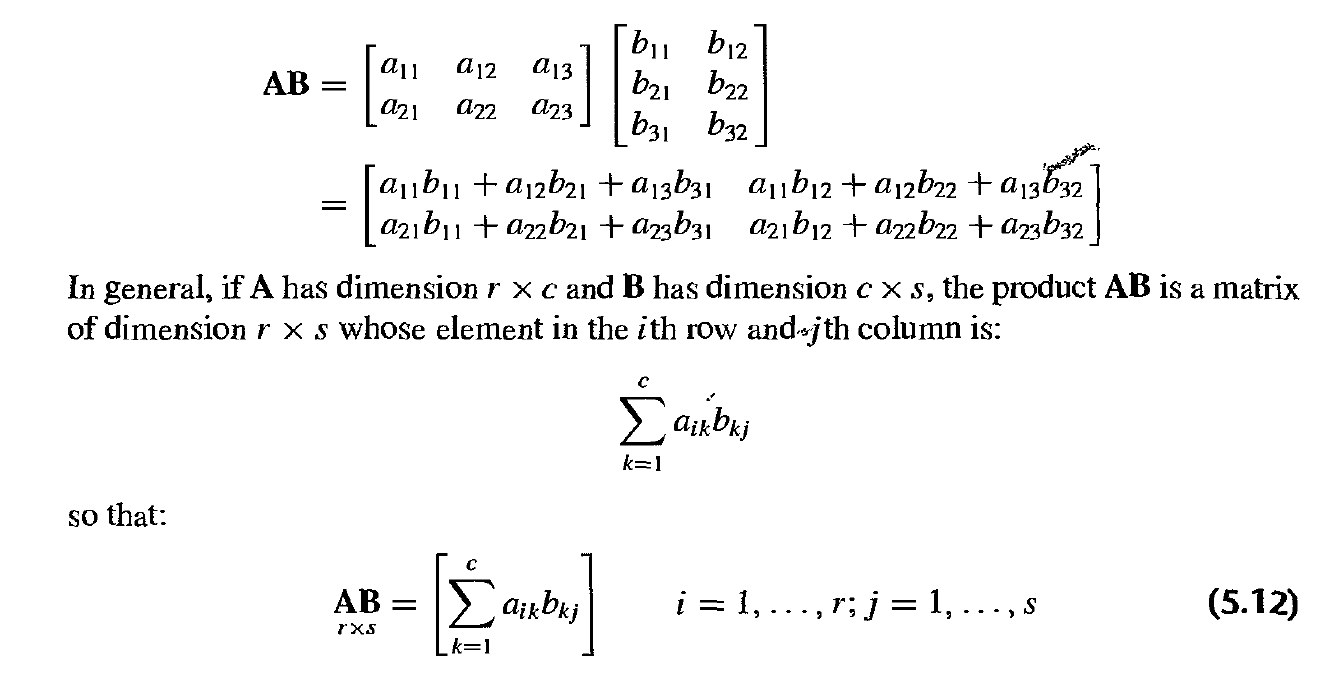
\includegraphics[width=1\linewidth]{resources/Class 02 - matrix multiplication} \end{center}

\end{frame}

\begin{frame}{Inverse of matrix}
\protect\hypertarget{inverse-of-matrix}{}

\begin{center}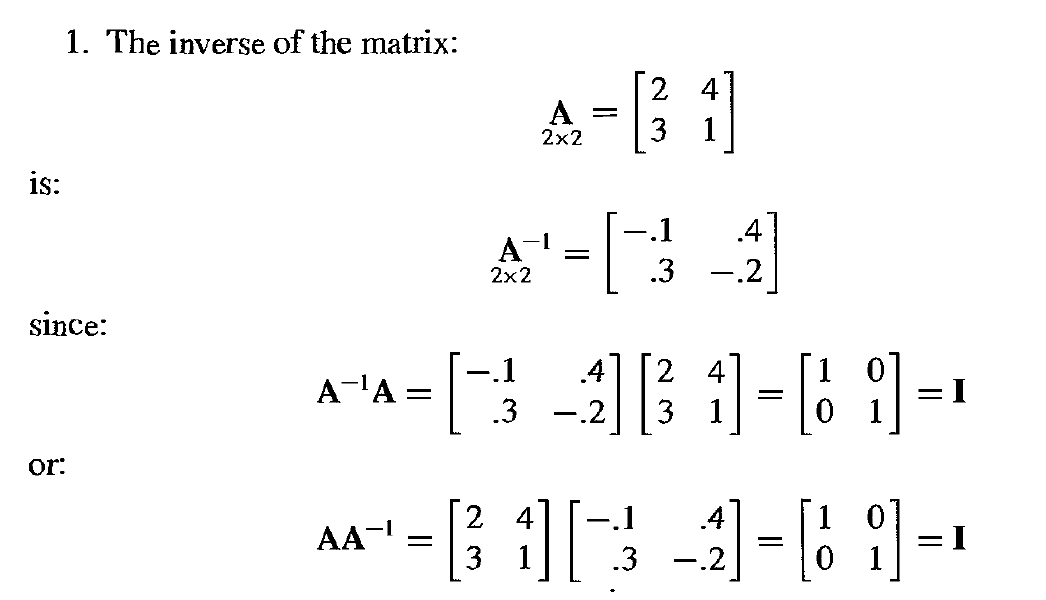
\includegraphics[width=1\linewidth]{resources/Class 02  - mm inverse} \end{center}

\end{frame}

\begin{frame}{Other Matrix Properties}
\protect\hypertarget{other-matrix-properties}{}

\begin{center}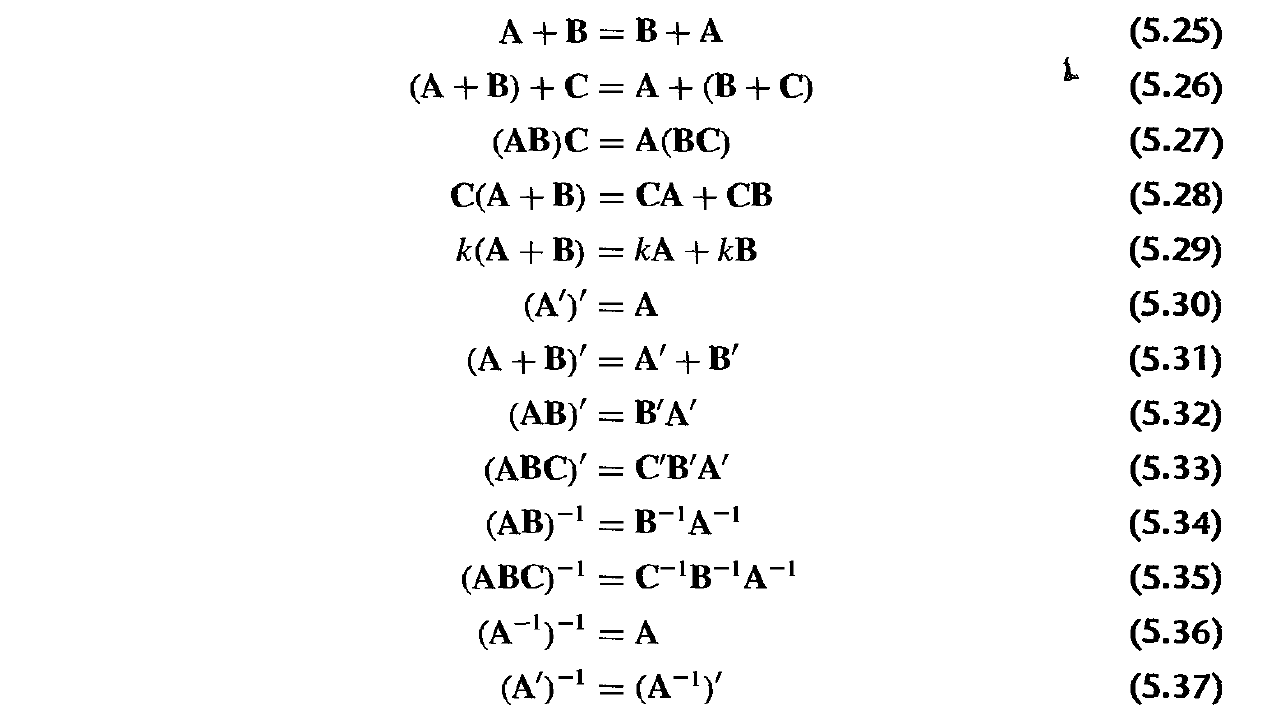
\includegraphics[width=1\linewidth]{resources/Class 02 - matrix props} \end{center}

\end{frame}

\begin{frame}{Variance-Covariance Matrix}
\protect\hypertarget{variance-covariance-matrix}{}

\begin{center}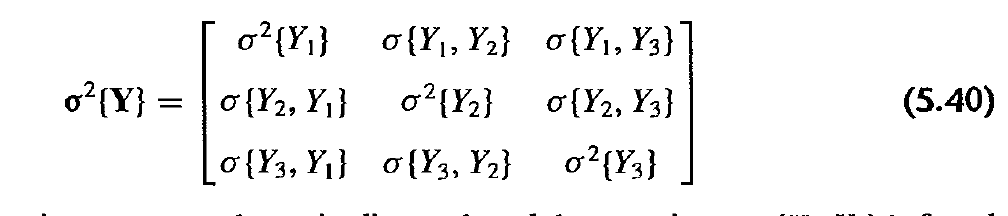
\includegraphics[width=1\linewidth]{resources/Class 02 - mm varcov} \end{center}

\end{frame}

\begin{frame}{Simple Model in Matrix Form}
\protect\hypertarget{simple-model-in-matrix-form}{}

\begin{center}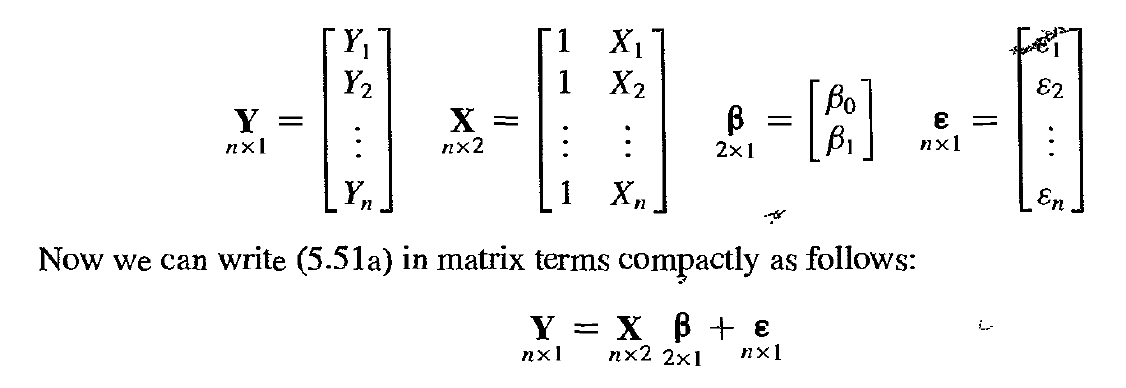
\includegraphics[width=1\linewidth]{resources/Class 02 - mm regression} \end{center}

\end{frame}

\end{document}
